% !TEX TS-program = pdflatex
% !TEX encoding = UTF-8 Unicode

% This is a simple template for a LaTeX document using the "article" class.
% See "book", "report", "letter" for other types of document.
\documentclass[12pt]{article} % use larger type; default would be 10pt

%\documentclass{amsart}
\usepackage[utf8]{inputenc} % set input encoding (not needed with XeLaTeX)
\usepackage{hyperref}
\usepackage{listings}
\usepackage{movie15}
\usepackage{graphicx}
\usepackage{tabu}

\hypersetup{
    colorlinks=true,
    linkcolor=blue,
    filecolor=magenta,      
    urlcolor=blue,
}

%%% Examples of Article customizations
% These packages are optional, depending whether you want the features they provide.
% See the LaTeX Companion or other references for full information.

%%% PAGE DIMENSIONS
\usepackage{geometry} % to change the page dimensions
\geometry{a4paper} % or letterpaper (US) or a5paper or....
% \geometry{margin=2in} % for example, change the margins to 2 inches all round
% \geometry{landscape} % set up the page for landscape
%   read geometry.pdf for detailed page layout information

\usepackage{graphicx} % support the \includegraphics command and options

% \usepackage[parfill]{parskip} % Activate to begin paragraphs with an empty line rather than an indent

%%% PACKAGES
\usepackage{booktabs} % for much better looking tables
\usepackage{array} % for better arrays (eg matrices) in maths
\usepackage{paralist} % very flexible & customisable lists (eg. enumerate/itemize, etc.)
\usepackage{verbatim} % adds environment for commenting out blocks of text & for better verbatim
\usepackage{subfig} % make it possible to include more than one captioned figure/table in a single float
% These packages are all incorporated in the memoir class to one degree or another...

%%% HEADERS & FOOTERS
\usepackage{fancyhdr} % This should be set AFTER setting up the page geometry
\pagestyle{fancy} % options: empty , plain , fancy
\renewcommand{\headrulewidth}{0pt} % customise the layout...
\lhead{}\chead{}\rhead{}
\lfoot{}\cfoot{\thepage}\rfoot{}

%%% SECTION TITLE APPEARANCE
\usepackage{sectsty}
\allsectionsfont{\sffamily\mdseries\upshape} % (See the fntguide.pdf for font help)
% (This matches ConTeXt defaults)

%%% ToC (table of contents) APPEARANCE
\usepackage[nottoc,notlof,notlot]{tocbibind} % Put the bibliography in the ToC
\usepackage[titles,subfigure]{tocloft} % Alter the style of the Table of Contents
\renewcommand{\cftsecfont}{\rmfamily\mdseries\upshape}
\renewcommand{\cftsecpagefont}{\rmfamily\mdseries\upshape} % No bold!

%%% END Article customizations

%%% The "real" document content comes below...

\title{EECS 233 HW9}
\author{Ben Pierce \\ \texttt{bgp12@case.edu}}
%\date{} % Activate to display a given date or no date (if empty),
         % otherwise the current date is printed 




%if anyone's reading this, any Latex tips/tricks would be greatly appreciated. 

\begin{document}
\maketitle
\title {GitHub: https://github.com/bp0017/CWRUEECS233/tree/master/HW9} 

\section{}
\subsection{A}
\begin{lstlisting}
C:\Users\bp001\Documents\EECS223\HW9>java Select
Here is the entire original array:
80  10  50  70  60  90  20  30  40  0
Selection sort...
[0][1][2][3][4][5][6][7][8][9]
80 10 50 70 60 90 20 30 40 0
80 40 50 70 60 90 20 30 10 0
80 40 50 70 60 90 30 20 10 0
80 40 50 70 60 90 30 20 10 0
80 90 50 70 60 40 30 20 10 0
80 90 60 70 50 40 30 20 10 0
80 90 70 60 50 40 30 20 10 0
80 90 70 60 50 40 30 20 10 0
90 80 70 60 50 40 30 20 10 0
\end{lstlisting}

\subsection{B}
\begin{lstlisting}
C:\Users\bp001\Documents\EECS223\HW9>java Insert
Here is the entire original array:
80  10  50  70  60  90  20  30  40  0
[0][1][2][3][4][5][6][7][8][9]
80 10 50 70 60 90 20 30 40 0
80 50 10 70 60 90 20 30 40 0
80 70 50 10 60 90 20 30 40 0
80 70 60 50 10 90 20 30 40 0
90 80 70 60 50 10 20 30 40 0
90 80 70 60 50 20 10 30 40 0
90 80 70 60 50 30 20 10 40 0
90 80 70 60 50 40 30 20 10 0
90 80 70 60 50 40 30 20 10 0
Final contents of the array:
90 80 70 60 50 40 30 20 10 0
\end{lstlisting}

\subsection{C}
\begin{lstlisting}
C:\Users\bp001\Documents\EECS223\HW9>java Mergesort
Here is the entire original array:
80  10  50  70
[0][1][2][3]
Dividing...
80 10  | 50 70
Dividing...
80  | 10
Merged
 80  10
Dividing...

Merged
 70  50
Merged
 80  70  50  10
 \end{lstlisting}
 \section{}
 \begin{lstlisting}
 C:\Users\bp001\Documents\EECS223\HW9>java Quicksort
Here is the entire original array:
1000  80  10  50  70  60  90  20  30  40  0  -1000
I have sorted all but the first and last numbers.
The numbers are now:
1000  0  10  20  30  40  50  60  70  80  90  -1000
\end{lstlisting}
\section{}
\subsection{A}
Selection sort can be implemented in two ways: from the left, or from the right.  I was taught from left to right, but in class, we did right to left, so I have included both.
\subsubsection{left-to-right}
\begin{tabular}{|c|c|c|c|c|c|}
\hline
10&60&40&50&30&20\\ \hline
60&10&40&50&30&20\\ \hline
60&50&40&10&30&20\\ \hline
60&50&40&30&10&20\\ \hline
60&50&40&30&20&10\\ \hline
\end{tabular}
\subsubsection{right-to-left}
\begin{tabular}{|c|c|c|c|c|c|}
\hline
10&60&40&50&30&20\\ \hline
20&10&40&50&30&10\\ \hline
30&60&40&50&20&10\\ \hline
50&60&40&30&20&10\\ \hline
60&50&40&30&20&10\\ \hline
\end{tabular}
\subsection{B}
\begin{tabular}{|c|c|c|c|c|c|}
\hline
10&60&40&50&30&20\\ \hline
60&10&40&50&30&20\\ \hline
60&40&10&50&30&20\\ \hline
60&50&40&10&30&20\\ \hline
60&50&40&30&10&20\\ \hline
60&50&40&30&20&10\\ \hline
\end{tabular}
\subsection{C}
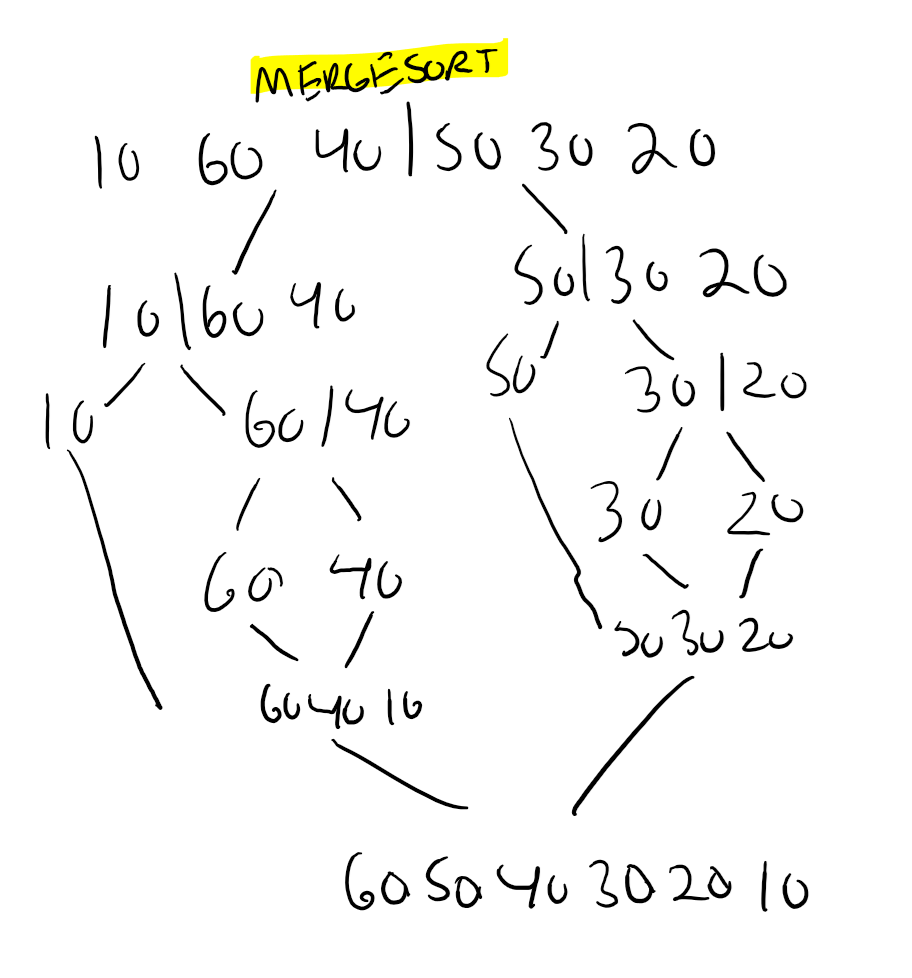
\includegraphics[scale=0.5]{mergesort.png}
\subsection{D}
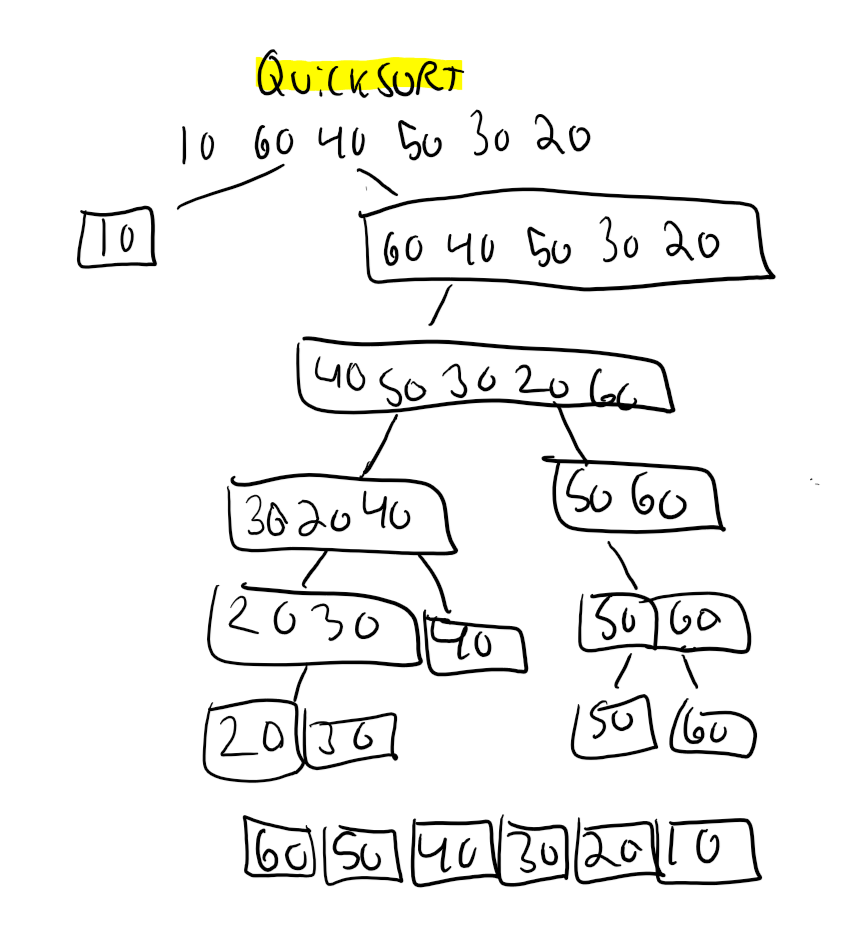
\includegraphics[scale=0.5]{quicksort.png}
\section{}
\subsection{A}
The average case for selection sort is $O(N^2)$, because the algorithim performs an inner loop and and outer loop roughly $N$ times, which results in an $O(N^2)$ Big-O time complexity. This can be derived by assuming that each the variable of iteration (usually i or j) is roughly equal to $N$; as the loops are nested, they are multiplied together in terms of time complexity. The expression for the time complexity is roughly $(N-1)(N)$, which reduces to $O(n^2)$
\subsection{B}
The average case for insertion sort is $O(N^2)$, due to having roughly $N^2$ shifts/compares in the average(and worst) case. As a general rule, an $O(n)$ algorithim inside a loop that iterates $N$ times is usually $O(N^2)$.
\subsection{C}
The average case for mergesort is $O(N*log N)$. The $log N$ component comes from the tree-like nature of the recursive calls, as the calls on the stack can be visualized as a tree with height $log N$. The merge is an $O(N)$ operation, and is done at every level. This makes mergesort an $O(N*log N)$ algorithim for the best, worst, and average case.
\subsection{D}
The average case for quicksort, like mergesort, is $O(N*log N)$. However, this runtime is dependent on the chosen pivot; a pivot chosen poorly can lead to an $O(N^2)$ performance from quicksort. However, with a correctly-chosen piviot, quicksort is $O(N*log N)$ for its average and best case.

\end{document}